\subsection*{\textbf{Задание 12.2} Построение нескольких графиков на дном изображении.}
\begin{itemize}
    \item Постройте в ожной системе координат графики следующиъ функций: $\sin[x^3], \sin[x], \cos[x], \sin[x]\cdot\x$ на отрезке $[-\pi,\pi]$.
    \item Укажите различные цвета для каждого графика.
    \item Настройте тип линии (например, пунктирная или точечная).
    \item Дайте название графику.
    \item Измените цвет фона с белого на любой другой.
    \item Пользуясб материалами лекции \textnumero5, сделать на графике цветные оси координат, выставить равные шкалы по осям,
    подписать оси, расставить необходимые метки по осям.
    \item Создать легенду.
    Для создания легенды воспользуйтесь справочной системой на команде Legend.
\end{itemize}

\begin{figure}[H]
    \renewcommand{\figurename}{Рисунок}
    \centering{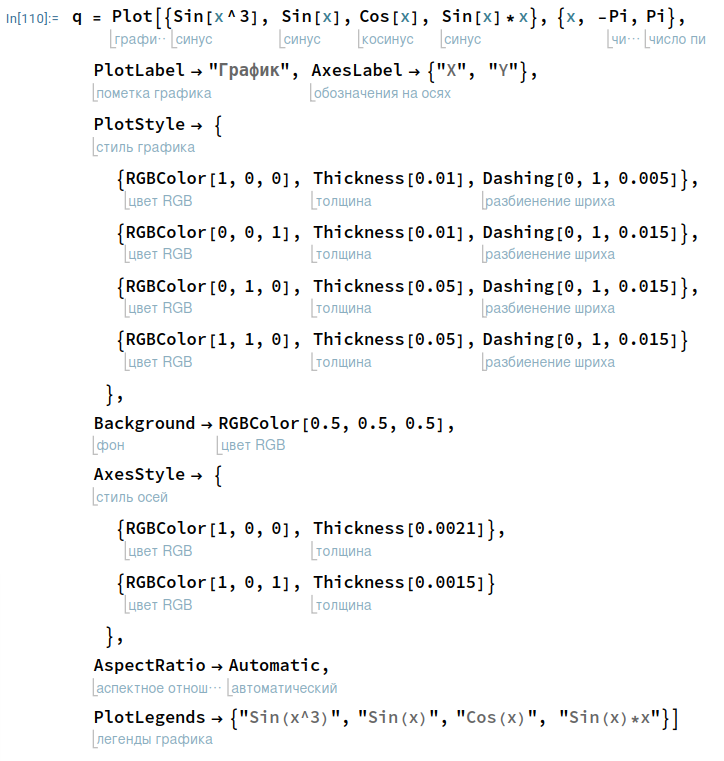
\includegraphics[scale=0.50]{body/img/12_2_1.png}}
    \label{fig:image_12_2_1}
\end{figure}

\begin{figure}[H]
    \renewcommand{\figurename}{Рисунок}
    \centering{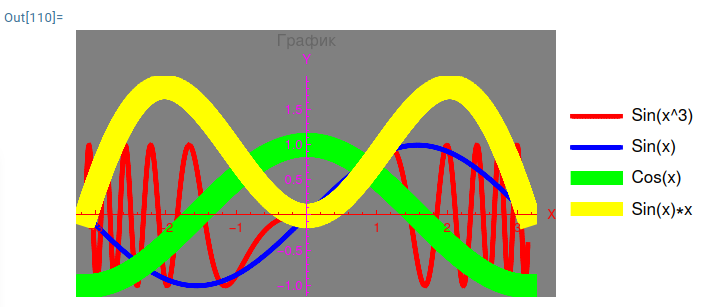
\includegraphics[scale=0.60]{body/img/12_2_2.png}}
    \label{fig:image_12_2_2}
\end{figure}